%All current and future systems.
%Economy of TRust
%Nominal Sets
%Hutton Heartbleed Hits email
%IAA
%Previous UK HoTT
%Nicola -> Awodey
%Visit Wadler
%Bib first names
%TXA observation citation
%WP relationships in S3
% Standardise Delivs and collabs
%Track records standfarise
% Refs: Pitts, Striecher, Hoffman, Als, Bauer, Uday, Rathjen, Escardo
% Changyu
%swwift
%HD vs proof relevant
%relatonships between wps

\documentclass[a4paper,11pt]{article}

\usepackage[top=2cm, bottom=2cm, left=2cm, right=2cm]{geometry}

\usepackage{mathptmx}
\usepackage{epsf}           %\input{epsf}
\usepackage{amsfonts}
\usepackage{amstext}
\usepackage{amssymb}
\usepackage{url}
%\usepackage[dvips]{graphics}
\usepackage[dvips,pdftex]{graphicx}
\usepackage[dvips,all]{xy}
\usepackage{multicol}
\usepackage{natbib}
\setlength{\bibsep}{0.0pt}

\usepackage{hyperref}

%\newlength{\extraplusheight}
%\newlength{\extrapluswidth}
%\setlength{\extraplusheight}{4.7cm}
%\setlength{\extrapluswidth}{4.7cm}
%\addtolength{\textwidth}{\extrapluswidth}
%\addtolength{\textheight}{\extraplusheight}
%\addtolength{\oddsidemargin}{-.5\extrapluswidth}
%\addtolength{\evensidemargin}{-.5\extrapluswidth}
%\addtolength{\topmargin}{-0.5\extraplusheight}
\setlength{\parindent}{0 pt}
\setlength{\parskip}{.5ex}

\newcommand{\eg}{{e.g.}\ }

\newcommand{\Int}[1]{[\![ #1 ]\!]}
\newcommand{\malign}[1]{\begin{array}[t]{@{}l@{\;}l@{}l@{}} #1 \end{array}}
\newcommand{\logrel}[2]{\Delta_{#1,#2}}
\newsavebox{\fminibox}
\newenvironment{fminipage}
 {\begin{lrbox}{\fminibox}\begin{minipage}{8cm}\vspace*{-2ex}}
 {\\[-2ex]\vspace*{-2ex}\end{minipage}\end{lrbox}\noindent\centerline{\fbox{\usebox{\fminibox}}}\vspace{0.5ex}}   

%\setlength{\parindent}{0.15in}
%\setlength{\parskip}{0.3ex}

% Discourage unnecessary hyphenation.
\sloppy\hyphenpenalty 4000

\newcommand{\ra}{\rightarrow}
\newcommand{\A}{\mathcal{A}}
\newcommand{\E}{\mathcal{E}}
\newcommand{\C}{\mathcal{C}}
\newcommand{\B}{\mathcal{B}}
\newcommand{\Set}{\mbox{{\sf Set}}}
\newcommand{\Nat}{\mathit{Nat}}
\newcommand{\Alge}[1]{\mathit{Alg}_{#1}}
\newcommand{\hash}{\#}

\begin{document}

\thispagestyle{plain}
\begin{center}
  {\Large {\bf Homotopy Type Theory: Programming and Verification}}\\[1ex] 

\vspace*{-0.1in}

%  {\Large \bf Case for Support}\\[1ex]
  \rule{140mm}{.5mm}\\[2ex]
\end{center}

\noindent
{\bf \Large Part 1A: Previous Research \& Track Record}

\textbf{Professor Neil Ghani.} Neil Ghani earned his PhD in Computer
Science in 1995 from the University of Edinburgh, where he worked on
categorical models of rewriting.  After becoming a Lecturer at
Leicester and then a Reader at Nottingham he was appointed to a
professorship at the University of Strathclyde where he founded the
Mathematically Structured Programming (MSP) group. His research has
focussed on a number of topics directly related to the subject of the
current proposal, \eg (1) his work on data types (containers, quotient
containers, indexed containers and induction recursion) is directly
related to our plans in WP3 to develop the theory of higher inductive
types; (2) his work on logical relations is directly related to our
plans in WP1 and WP2 to develop the model theory for HoTT as well as
the syntactic presentation of this model theory as a type theory; (3)
his work on the semantics of effects is directly related to the
application of HoTT to effects as planned in WP4; and (4) his work on
Units of Measure (via an IAA grant held in collaboration with
Microsoft) directly relates to WP8 which applies HoTT to computing
with algebraic structures such as within Units of Measure. Indeed,
results obtained during his previous EPSRC grants on Containers,
Induction Recursion and Logical Relations will feed into this
proposal.  More generally, Neil Ghani is a world expert on the use of
semantic structures to drive the development of type theory and
programming languages, exactly the methodology to be followed in this
proposal.

Professor Ghani serves as a member of the EPSRC College charged with
assessing the quality of grant applications. He is also a grant
assessor for the Carnegie Trust.  He was the director of the Midlands
Graduate School in the Foundations of Computer Science, is a SICSA
theme leader in Complex Systems Engineering, and was on the Steering
Committee for the British Colloquium on Theoretical Computer Science.
He has served on numerous programme committees and been the external
examiner for a number of PhD students. He is also Deputy Head of
department and Head of Research in his home Department. He has
successfully supervised five PhD students and four RAs and has
experience in the successful management of large grants. He organises
the Scot Cats seminar series, and plans to host a meeting in the UK on
Homotopy Type Theory in November 2014, both of which puts him in touch
with other experts in the area.

For further information, see~\url{http://www.cis.strath.ac.uk/~ng}

\textbf{Dr Conor McBride.} Conor McBride received his PhD from the
University of Edinburgh in 1999 for his work on dependently typed
programming. After this, he worked as an RA at the Universities of
Durham and Nottingham before becoming a lecturer at the University of
Strathclyde in 2008. His work on the foundations and implementations
of non-dependently and dependently typed programming as become very
influential, both via his own programming language Epigram and via his
work with the Agda, Coq and Haskell teams. He is now widely regarded
as a leader of his field as illustrated by his widely cited papers,
journals, and invitations to keynote addresses at conferences
etc. Apart from the evident importance of this expertise for WP6 and
WP7, Dr McBride's work on OTT, on containers and on effects feed into
WPs 3 and 4. Since becoming a lecturer, Dr McBride has had two grants
funded by EPSRC and - importantly - one by Microsoft. Not only are all
of these grants of direct relevance to this project, but these grants
show both his experience of working in large distributed grants and
that our plans for generating industrial impact through collaborations
with Microsoft are built on solid and successful pre-existing
foundations. Dr McBride has also supervised two PhD students and
currently supervises a further two students. He also leads the MSP
group.

For further information,
see~\url{https://personal.cis.strath.ac.uk/conor.mcbride/}

\textbf{Host Institution: The University of Strathclyde.} The MSP
group at the University of Strathclyde is an ideal venue for
conducting this research. Led by Conor McBride, the group includes
Prof Ghani, Dr Clemens Kupke, Dr Ross Duncan as well as two research
associates and seven PhD students. The MSP groups vision is to use
mathematics to understand the nature of computation, and to turn that
understanding into the next generation of programming languages. That
is exactly the methodology used within this proposal and hence this
proposal will both benefit from, and benefit, the MSP group.
Finally, central Scotland is home to vibrant theoretical computer
science and functional programming research communities, and the
University of Strathclyde is an active participant in the Scottish
Informatics and Computer Science Alliance (SICSA). The MSP group also
is active in other Scottish meetings, such as ScotCats and SPLS.

\newpage
\textbf{Dr Thorsten Altenkirch.}  Thorsten Altenkirch received his PhD in
Computer Science from the University of Edinburgh in 1993. Since 2006
he is Reader at the University of Nottingham,
where he founded the Functional Programming Laboratory with Graham
Hutton in 2008. Altenkirch is well known for his work on type theory
and applications of category theory in computer science, and has
published over 50 research papers which are frequently cited (h-index~$\geq 26$). During his
work at Nottingham he attracted \pounds 1M in research funding,
comprising~\pounds650,903 as PI in 4 EPSRC grants, \pounds241,075 as
CoI in 2 EPSRC grants, \pounds159,038 in 1 fellowship and 1
studentship. Especially relevant for the current project is
Observational Equality For Dependently Typed Programming
(EP/C512022/1), Theory And Applications of Induction Recursion
(EP/G03298X/1), Reusability and Dependent Types
(EP/G034109/1). Altenkirch and Ghani have already collaborated
successfully on three research grants. More generally, 
Altenkirch is one of the leading researchers on HoTT
This is witnessed by his fellowship at the Institute of Advanced Study
in Princeton in occasion of the special year on the subject in 2013. There, he contributed to the standard reference on the
subject~\cite{hott-book}.  He has given invited lectures on the
subject (at HDACT in Lubljana in 2012, at the Curien-fest in Venice in
2013, at MSC in Lyon and at the Institut Henri Poincar\'e in Paris in
2014 \cite{txa-ihp14}). He has already published several papers on HoTT
\cite{altenkirch:extSetoids,alti:ott-conf,alti:csl12,alti:tlca13-hedberg}.

For further information, see~\url{http://www.cs.nott.ac.uk/~txa}

\textbf{Host institution: The University of Nottingham.}  The
University of Nottingham is a leading UK University 
and its School of Computer Science was ranked 8th in the last Research
Assessment Exercise. The Functional Programming Lab (FP Lab) within the School
is one of its four major research groups, with an international
reputation for its work on formally-based approaches to software
construction and verification.  The FP Lab currently comprises 4
academic staff: Professor Graham Hutton, Dr Thorsten Altenkirch, Dr
Venanzio Capretta, and Dr Henrik Nilsson and nine PhD students.  To
date, the group has received~\pounds1.5M of EPSRC funding over 14
projects, and has 12 completed PhD students.  The FP Lab provides a highly stimulating research environment,
holds weekly research seminars and is also a leading participant in the MGS - a
collaborative venture with Leicester and Birmingham offering training
to PhD students.
\noindent

\textbf{Dr Nicola Gambino.} Nicola Gambino received his PhD in
Computer Science from the University of Manchester in 2002. After
carrying out postdoctoral research, he became an Assistant Professor
in Mathematical Logic at the University of Palermo in 2008. Since
 2012, he is an Associate Professor in Pure Mathematics at
the University of Leeds. Nicola Gambino has a consistent record of
publications in leading journals and of invited lectures at
international conferences, {e.g.}~at the 2010 Logic Colloquium in Paris
and at the forthcoming joint 2014 RTA-TLCA conference in Vienna. He
held visiting positions at several prestigious research centres, including the Institut Mittag-Leffler (Stockholm), the
Fields Institute (Toronto) and the Institute of Advanced Study
(Princeton), where he worked in contact with Vladimir Voevodsky (the inventor of 
the Univalence Axiom).  He is currently an invited researcher to the
Institut Henri Poincar\'e (Paris) for the special trimester on
Semantics of Proofs and Certified Mathematics.  He is an editor of the
journal Mathematical Structures in Computer Science. He has been funded by 
EPSRC via a Postdoctoral Fellowship in Mathematics (GR/R95975/01), held at the University of Cambridge. He is currently PI on a grant from 
the US Air Force Office for Scientific
Research, which is funding an RA working on the relation between HoTT and
higher-dimensional category theory. 
Nicola Gambino is one of the leading researchers on HoTT; in particular, in collaboration with Richard Garner, he obtained~\cite{gambinoGarner:ITwfs} one of the 
very first results relating type theory and homotopy theory. His work in HoTT, \eg \cite{awodeyGamSoja:indTypesInHTT}, builds on his combination of expertise in type theory~\cite{GambinoN:gentti}, category 
theory~\cite{gambinoHyland:welfoundedTrees,GambinoN:polfpm} and homotopical algebra~\cite{GambinoN:homl2c,GambinoN:weilsh}.





For further information,  see~\url{http://www.maths.leeds.ac.uk/~pmtng}.

\textbf{Host Institution: The University of Leeds.} The University of
Leeds is a leading UK university providing
excellent facilities for research. The School of Mathematics hosts the
Mathematical Logic group, including seven members of staff, four
research fellows and nineteen research students. The group has a
vibrant research profile; it frequently organises
international conferences and runs several regular activities,
including a weekly Mathematical Logic Colloquium and specialist
seminar series on model theory, proof theory and computability
theory. The Mathematical Logic group has been consistently funded by
EPSRC and international agencies and is already active on Homotopy
Type Theory. In particular, we intend to collaborate closely with
Professor Michael Rathjen who is currently PI
on a 3-year EPSRC grant on proof-theoretical aspects of HoTT. 


\newpage
\noindent
{\bf \Large Part 2: The Proposed Research and Its Context}

\vspace*{-0.23in}

\begin{center}
\rule{170mm}{.5mm}
\end{center}

\vspace*{-0.4in}

\section{Introduction}\label{sec:intro}

\vspace*{-0.1in}

{\bf Formal Verification.} The cost of software failure is truly
staggering\footnote{see the section on National
  Importance.}. Traditional methods of software verification based
upon testing only generate partial guarantees of correctness and
although stronger
guarantees of software correctness can be given by mathematical
proofs, the complexity of modern software means that hand written
mathematical proofs are untrustworthy. Indeed, the only way to
ensure truly secure and reliable software is the gold standard of
formally verified software, which offers machine-checked mathematical
proofs of software correctness. Several decades of pioneering work in
the UK and elsewhere has culminated in systems 
such as Agda, Coq, Epigram, Idris, NuPRL, Twelf, and
the Trellys project which are now having significant impact,
\eg Coq has won both the 2013 ACM Software award and the 2013 SIGPLAN
Programming Languages Software award. The advanced type-theoretic
technology of these systems is also raided by more mainstream languages
with significant industrial deployment such as Haskell, OCaml, Scala
and C\#.

%SWIFT
%Other prizes for other systems
%Economy of Trust

{\bf The Project.} Despite their success, such systems have several
fundamental limitations, \eg when programming with quotients,
supporting abstraction (that is, invariance under different
representations of the same structure) and extensional reasoning
(proving that programs which behave the same are the same).  {\em
  Homotopy Type Theory} (HoTT) is widely regarded as a fundamental
innovation with great potential to address these and other problems.
To realise this potential, we propose a synthesis of
theoretical, applied and impact-focussed research.


%Delivering this potential requires i) further development of the
%foundations of HoTT; ii) programming language and verification tools
%based on these foundations; and iii) applications demonstrating their
%effectiveness to the broader community.  Therefore we i
%The key concept in HoTT is to introduce a very liberal
%equality which identifies structures that are replacable.

%Its core is Voevodsky's {\em Univalence Axiom} asserting
%that all provable equalities can be internalised as paths or, more
%conceptually, that computation is invariant under change of
%representation of the entities we compute with.


$\;\;\; \;\;\;$ {\em Theoretical Foundations.} Almost all of our
understanding of HoTT exists within a classical framework and hence
cannot be used to develop programming language and verification
tools. However, the recent cubical sets model by Coquand
et.al.~\cite{BezemM:cubsmt} is constructive and thus strongly suggests
that HoTT has a
purely constructive presentation. We will develop
both specific constructive 
models 
and a general constructive model theory 
of HoTT, and then complement these models with type theoretic
presentations of them.

$\;\;\;\;\;\;$ {\em Programming Language and Verification Tools.} The key
  deliverable of the second strand of our research is a HoTT-based
  programming language which simultaneously acts as a verification
  environment. This will translate the fundamental innovation of HoTT
  into a fundamental innovation within programming languages
  which will influence
  the development of all current and future systems in this area.

$\;\;\;\;\;\;$ {\em Generating Impact.} Developing new and fundamentally
  better ways to construct formally verified software is not just an
  end in itself, but is also a key prerequisite for engaging others to
  do the same.  To ensure this, we will produce a number of case studies so
  users can learn from, and experiment with, our results. Their
  practical experiences will also feed back into our research.

  {\bf Calibre, Ambition, and Adventure.} HoTT's potential to
  solve one of the deepest and most fundamental problems in
  programming languages and verification - namely the efficient
  computational treatment of equality/representational invariance -
  demonstrates our ambition to transform the field. The proposal's calibre is demonstrated by
  the depth and range of the state-of-the-art ideas deployed and by the
  stature of our collaborators. The
  proposal's adventure is demonstrated by its scope, ranging from
  fundamental research (WP1,2,3) to programming languages and
  verification (WP5,6,7) to impact generation via case studies
  (WP4,8).

\vspace*{-0.1in} 

% %txa: added heartbleed.
% %{\bf Cost of Software Failure:} The cost of software failure is truly
% %staggering. Well known individual cases include the Mars Climate
% %Orbiter failure ($\pounds 80$ million), Ariane Rocket disaster
% %($\pounds 350$ 
% %million), Pentium Chip Division failure ($\pounds 300$ million), most recently
% %the heartbleed bug (upto $\pounds 250$K per server) and there are
% %many, many more examples. Even worse, other software failures such as
% %one in the Patriot Missile System and another in the Therac-25 radiation system
% %have costs lives. More generally, a 2008 study by the US
% %government estimated that faulty software costs the US economy
% %$\pounds 40$ billion annually.  As a result, the human and economic
% %importance of ensuring programs run without error is hard to
% %over-estimate.
 

% %The worldwide software market is estimated at
% %\pounds 250 billion pounds every year and this figure will grow
% %significantly in real terms as software becomes ever more ubiquitous
% %in our lives and economy. Although the requirements for software vary
% %enormously, a problem common to all software is to ensure programs run
% %without error. Restarting a phone is a simple, if inconvenient task;
% %restarting an aeroplane in mid-flight is not an option! Numerous
% %examples of expensive software errors about from the Mars Rover to be
% %recent Heartbleed Bug exposing a serious vulnerability in the popular
% %OpenSSL cryptographic software library.  In a nutshell, the cost of software bugs is almost
% %unbelievably staggering.

% {\bf Formal Verification.} The cost of software failure is truly
% staggering\footnote{see the section on National
%   Importance.}. Traditional methods of software verification based
% upon testing only generate partial guarantees of correctness. Stronger
% guarantees of software correctness are given by mathematical proofs
% but the complexity of modern software means that hand written
% mathematical proofs are untrustworthy. As a result, the only way to
% ensure truly secure and reliable software is the gold standard of
% formally verified software, which offers machine-checked mathematical
% proofs of software correctness. Several decades of pioneering work in
% the UK and elsewhere have culminated in prototype languages and tools
% such as Agda, Epigram, Idris and Coq and in the US NuPRL, Twelf, and
% the Trellys project. These systems are beginning to make their mark,
% \eg Coq has just won both the ACM Software award and the SIGPLAN
% Programming Languages Software award.
% %~\cite{}.  -not needed, txa
% The advanced
% type-theoretic technology of these systems is raided by more
% mainstream languages with significant industrial deployment such as
% Haskell, OCaml, Scala and C\#.

% {\bf The Project.} Despite these successes, such systems have a number
% of short comings in crucial areas, \eg when programming with quotient
% types, supporting abstraction (that is, invariance under different
% representations of the same structure) and extensional reasoning
% (proving that programs which behave the same are the same).  {\em
%   Homotopy Type Theory} (HoTT) is widely regarded as a fundamental
% innovation with great potential to address these and other problems.
% Delivering this potential requires i) further
% development of the foundations of HoTT; ii)
% a programming language and verification environment based on
% these foundations; and iii) applications demonstrating the effectiveness
% of this environment to the broader software development community.
% Therefore we intend to pursue a three-pronged
% research programme based upon a synthesis of theoretical, applied and
% impact-focussed research.

% %The key concept in HoTT is to introduce a very liberal
% %equality which identifies structures that are replacable.

% %Its core is Voevodsky's {\em Univalence Axiom} asserting
% %that all provable equalities can be internalised as paths or, more
% %conceptually, that computation is invariant under change of
% %representation of the entities we compute with. 



% \begin{itemize}
% \item {\bf Theoretical Foundations.} Almost all of our understanding
%   of HoTT exists within a classical framework and hence cannot be used
%   to develop programming language and verification tools. Nevertheless, the recent
%   work by Coquand et al. strongly suggests a constructive presentation of HoTT
%   is possible. We will develop both specific constructive models
%   and a general constructive model theory of HoTT, and then complement
%   these models with type theoretic presentations of them.
% \item {\bf Programming Languages and Verification:} The key
%   deliverable of the second strand of our research will be a
%   programming language which simultaneously acts as a verification
%   environment based upon HoTT. This is likely to become a major
%   step forward in programming languages design and influence
%   the development of all current and future systems in this area.
% \item {\bf Generating Impact:} Developing new and fundamentally
%   better ways to construct formally verified software is not just an
%   end in itself, but is also a key prerequisite for engaging others do
%   do so.  To help ensure uptake of our research by the wider
%   community, we will produce a number of case studies which will allow
%   users to experiment with our results; at the same time, their
%   practical experiences with it will feed back into our research.
% \end{itemize}

% {\bf Calibre and Ambition.} The foundational nature of HoTT, the
% consequent potential for solving key open problems in programming
% languages and formal verification research, and the resulting
% potential applications to software correctness attest to the quality
% and calibre of this project. Our ambition is demonstrated by the
% breadth of our central belief that HoTT is not just a mathematical
% foundation for type theory, but can also be turned into a programming
% language and verification environment which - in its treatment of
% quotients, representational invariance and equality - will become the
% benchmark standard which current and future systems will seek to
% emulate.

\vspace*{-0.1in} 
\section{Scientific and Technological Background.}
\vspace*{-0.1in} 

{\bf Programming Languages.} Abstraction is essential in programming
as identifying common structure ensures code is clear,
clean and concise. This leads to high level
programming languages with expressive type systems capable of closing
the {\em semantic gap} between what programmers know about
computational entities and what their types can express about them.
The current state-of-the-art are the {\em dependently typed
  programming languages} mentioned above where
the type of a program can express a
continuum of precision - from basic assertions up to a complete
specification - about the program's behaviour. This proposal will
develop the first of a new breed of 
such languages which advance the state-of-the-art by offering a
powerful yet computationally tractable equality, and thereby bring to
reality the goal of programming up to invariance of representation.

%Coq award
%transform
%ahead of the curve

{\bf Program Verification.} While the advantages of the certainty
afforded by mathematical proof has been recognised for centuries, this
certainty is undermined by the capacity for humans to make mistakes in
proofs. The advent of computers raised the possibility once more of
achieving in practice the promise of mathematical certainty. This
potential is now coming to fruition, \eg systems such as Coq have been
able to formally verify both large mathematical theorems such as the
4-Colour problem, and large software systems such as the CompCert
C-compiler. However, these systems are not {\em extensional}:
behaviourally indistinguishable objects cannot be proven to be the
same and this fundamental problem significantly weakens the system's
usability. We will rectify this by producing a system where
objects with the same behaviour can indeed be proved equal.


{\bf Type Theory.} Underlying formal verification systems and
programming languages is the subject of type theory. The
Curry-Howard correspondence asserts that programs and proofs are
actually the same thing, \eg proofs are just particular forms of
programs - developing sophisticated type theories thus advances both 
the fields of programming and verification. Another
major advance was Martin-L\"of's realisation that type theory needed
%to be extended 
to cover equality - however, although 
extensional Martin-L\"of Type Theory produced
a strong equality, it had the fundamental flaw that type
checking was undecidable. He then formulated intensional Martin-L\"of
Type Theory (MLTT) but its equality proved to be too weak, \eg
pointwise equal functions cannot be proven equal. Defining a strong yet
computationally tractable equality has remained unresolved for 40
years - HoTT is so exciting precisely because it offers a
solution to this most fundamental of problems.

{\bf Observational Type Theory (OTT) and Logical Relations:} OTT was
proposed by Altenkirch and McBride~\cite{alti:ott-conf} as a step
towards such a stronger equality. While the equality type of MLTT is
defined uniformly over types, OTT defines an extensional and
decidable equality by induction on the type structure. However, the
{\em equality of types} themselves is rigidly structural preventing 
conversion of proofs about one type into proofs about an equivalent type. As
HoTT can be seen as a proof-relevant extension of OTT, our experience
in OTT will be invaluable.
% throughout the project. 
Logical relations also use induction on type structure
to define not equalities, but rather relations, over all
types. They have already been
used~\cite{licataHarper:canonicity2d} to study a truncated form of
HoTT. Further, cubical sets~\cite{BezemM:cubsmt} 
arise naturally when one extends logical
relations to higher dimensions via the pattern of set, relation,
relation between relations etc. Ghani's EPSRC-funded research on
logical relations will be used to inject advanced logical relations
ideas, \eg higher dimensional logical relations, throughout
the project.


%power of methods
%absolutely vital
%very clear evidence

% invariance of representation = iso == equal
%vs
% strength of propositional equality (= identity type)
% strength of definitional equality beta

% hott or univalence
% hott = tt + univalence + hits
% univalance + hdtt/hdct
% hott = int param + kan filllers + hits
% what does univalence mean

{\bf Homotopy Type Theory.} HoTT is a revolutionary new understanding of
type theory based on intuitions from homotopy theory. Types are
\emph{spaces}; terms are \emph{elements} within a space; the equality
type is the space of \emph{paths} in a space. Such paths contain
non-trivial structural information enabling us to program and reason up to invariance of
representation. The core of HoTT is the new Axiom of Univalence,
introduced by Fields medalist Vladimir Voevodsky, asserting (roughly)
that isomorphic types are equal. HoTT subsumes function extensionality
but also transcends what we could previously express, e.g.\
\emph{higher} inductive types (HITs) include the usual tree-like data
types, but also include quotients \cite{alti:mpc04} and geometric
objects such as the circle and sphere. HITs also occur in computer
science, e.g. lists are an inductive type; braids are lists with extra
paths identifying lists up to twisting of any element past its
neighbours, and bags are braids with paths-between-paths identifying
braidings which yield the same permutation. 
The interpretation of closed expressions of HoTT within the cubical
sets model~\cite{BezemM:cubsmt} proves the basic feasibility of computing
with the Univalence Axiom. However, much work remains: closed
expressions  must be interpreted  \emph{within} HoTT itself and 
not just within the model. Definitional equalities lost by the cubical interpretation (such as
the computation rule for equality types) must be recovered. Further, other models may
offer better computational foundations for HoTT, so practical progress
towards HoTT-based programming languages and verification tools needs
the broader model theory we propose.



%txa: replacing
% One of the key features of Coquand's model is that
% the equality relation is defined recursively over the structure of
% types using an internalised form of parametricity. 




% Nevertheless, Coquand's and Huber's
%work shows that producing programming languages and proof assistants
%based upon HoTT is feasible in principle and we plan to
%collaborate closely with them.


%Earleir motivation for OTT
%Grant numbers below

%Mention somewhere the prizes that Coq has been recently been awarded, as proof that this is cutting-edge technology

%Mention somewhere that HoTT is having an impact on the design of (new versions of) Coq: there is ongoing work on implementing mechanisms for higher inductive types (Barras). Also: Bauer is working on new proof assistant based on ideas of Voevodsky.

%Mention somewhere also the importance of type theory, Coq, Agda for
%computer-assisted formalization of mathematical proofs 

%Why us and not the United States of Awodey. Strong definitional
%equlity. 

\vspace*{-0.2in}

\section{Methodology and Research Programme}
\vspace*{-0.1in}

Our methodology harnesses ideas from i) our experiences and
competencies -- see our track records and the {\em
  Justification of Resources}; and 
%different sources: i) our work on logical relations and on OTT
%which can be seen as proof-irrelevant variants of what we propose; ii)
%our work on the implementation of dependently typed programming
%languages (Epigram and $\Pi\Sigma$
%\cite{alti:pisigma-new,alti:checking}); iii) our work on datatypes
%(containers, indexed containers, induction-induction and
%induction-recursion)
%\cite{alti:fossacs03,alti:tlca03,alti:icalp04,alti:jpartial,alti:mpc04,alti:cont-tcs,alti:regular,alti:cats07,alti:jcats07,alti:lics09,
 % alti:catind2}; iv) our work on constructing internal models of type
%theory; and 
ii) the evolving state-of-the-art, our ongoing dialogue with our
world leading collaborators, and the workshop/events we intend to
organise/attend to foster interaction. These multiple sources ensure that we neither
slavishly follow the hype that inevitably surrounds such a significant
innovation, nor are unaware of current and future advances. The
project is structured as follows:

%divided into eight work packages, each having a named collaborator, a clear deliverable of
%relatively low risk (to ensure the overall project's success) as well
%as a more ambitious goal:

%with WP1
%hosted in Leeds, WP2-4 in Nottingham and WP5-8 in Strathclyde. Of course
%the reality is that we will continue our established practice of
%working closely together.

%Argue in justification for resources
%Explain compute below 



{\bf WP1: Semantic Foundations of HoTT.}  %We seek semantic insights
%for HoTT akin to those provided by Cartesian closed categories for
%the simply typed $\lambda$-calculus.  
A proper model theory for
HoTT is essential because i) a general model theory 
guides the design of different presentations and implementations of
HoTT; ii) models of HoTT provide algebraic techniques to reason
about the correctness of implementations which complement syntactic
techniques; and iii) specific implementations of HoTT can
be proven sound by giving a specific models of them.  These models
need to be constructive so that all programs reduce to a normal form.
%While
%the standard model of HoTT based upon simplicial sets is not
%constructive, the cubical sets model currently being developed~\cite{BezemM:cubsmt} is constructive and raises the question of understanding it
%within a general model theory.
We will: i) analyse existing models ({e.g.}
groupoids~\cite{HofmannM:groitt}, simplicial
sets~\cite{KapulkinC:simmuv}, cubical sets~\cite{BezemM:cubsmt}) and
isolate exactly how they ensure constructivity or where they fail to
do so - in the latter case, we will attempt to constructivize them;
ii) building on this, we will develop a general model theory for HoTT
by isolating the essential features of these models and by adapting
known methods to construct Quillen model structures to the setting of
HoTT ({c.f.}~\cite{ShulmanM:uniidh}, which however does not cover the
cubical sets model).  The challenge is to take the recent advances in
axiomatizing models of type theory
({e.g.}~\cite{AwodeyS:natmtt}) and blend in the additional structure of HoTT. In terms
of risk, i) is certainly achievable as it involves only the
analysis of existing concrete models, while ii) is a more ambitious
goal. Nevertheless, our expertise on semantics of type
theories~\cite{neil2014relParamDep}, homotopical
algebra~\cite{GambinoN:homl2c,GambinoN:weilsh} and
$\omega$-groupoids~\cite{alti:csl12} makes even this ambitious goal
feasible. {\em Deliverables: A broad collection of models of HoTT
  which mapping the design space of its syntactic
  presentations. Collaborator: Steve Awodey.}



% {\bf WP1: Semantic Foundations of HoTT:}  We
% seek semantic insights into HoTT akin to those provided by Cartesian
% closed categories for the simply typed
% $\lambda$-calculus.  A constructive model theory for HoTT is essential because: i)
% specific implementations of HoTT can be proven sound by giving a specific
% models of them; ii) 
% %since we don't know a priori what the best implementation
% %of HoTT will be, 
% a general model theory of HoTT will implicitly predict, and thereby
% guide, the design space of different presentations and implementations
% of HoTT; and iii) models of HoTT will provide algebraic techniques to
% reason about the correctness of implementations which complement
% syntactic techniques. These models need to be constructive so that
% programs, even those using Univalence, will compute. While the
% standard model of HoTT based upon simplicial sets is not constructive,
% Coquand et al.'s recent cubical set model is constructive and 
% has thus opened the door to a more general model theory.

% %Joyal
% %Back ground : Qullien model structures

% We will attack this problem from the following directions: i) we will
% analyse existing models (cubical sets, groupoids, strict
% $\omega$-groupoids, simplicial sets, globular sets) to isolate exactly
% how they ensure constructivity, or (where they fail to do so) how to 
% constructivize them; and ii) informed by i),
% we will develop a model theory for HoTT by both adapting known methods to
% define Quillen model structures (such as the small object argument)
% to the constructive setting and by showing how one can build  new
% constructive model structures from old (\eg by
% slicing). A promising starting point for a constructive
% version of the small object argument comes from Garner's work, where
% it is related to the construction of free monads. In terms of risk,
% i) is certainly achievable since it involves only the analysis of
% existing concrete models, while ii) is a more ambitious
% goal. Nevertheless, our expertise on semantic models of parametricity \cite{neil2014relParamDep}, model
% categories (Gambino) and $\omega$-groupoids \cite{alti:csl12} makes even this
% ambitious goal feasible. Deliverables from WP1 will be a broad class
% of models of HoTT which considerably deepen our
% understanding and map out the design space of its 
% syntactic presentations.

% back ground work: NOMINAL SETS,

%LARGE BODY OF
%WORK ON SIMPLICIAL SETS AND MODEL CATEGORIES. MANY MODELS =>
%UNIVERSALLY VALID PRINCIPLES.
% Design space of the HoTT family earlier om

%Background: current presentation (HoTT presentation and Thierry's)
%dont have canonicity.

{\bf WP2: Univalent Type Theory.} Building on WP1, we need syntactic
presentations of our models of HoTT in the form of type theories. The
challenge is to present the essential data of the model as built from
a {\em finite} collection of type and term constructors - this is
particularly intricate given the {\em arbitrary} higher dimensional
structure of HoTT. One also must prove essential properties such as strong normalisation, decidability of
definitional equality and canonicity (i.e. all terms reduce to
values). It is of particular interest to establish the expressive
power of the associated equational theories, e.g. to distinguish
carefully between which computation rules hold as definitional
equalities and which as propositional equalities. Another key property
(required for WP5) is that, as a foundational theory, our type theory
ought to be expressive enough to describe its own models. These
properties will be established either directly or via the models of
WP1.
%Different models will produce different theories and we
%will analyse them in terms of their tractablility, concision and 
%meta-theoretic properties. Essential properties we require of a well
%behaved type theory are
% We will begin by developing Altenkirch's preliminary type theory for
% cubical sets, which both internalises parametricity and adds Kan
% fillers to the theory. 
We will build on Altenkirch's observation \cite{txa-ihp14} that cubical sets share
many similarities with logical relations by replacing the uniform
identity type of intensional MLTT with a higher-dimensional equality
defined to fit the structure of types. The models from WP1 will drive
refinement of our design, until we have a canonical presentation of
HoTT. Our preparatory work~\cite{txa-ihp14}, and prior expertise in OTT
\cite{alti:ott-conf}, normalisation by evaluation and big-step
reduction \cite{alti:ctcs95,alti:lics96,alti:flops04,txa:jtait},
strengthening definitional
equality~\cite{Allais:2013:NEN:2502409.2502411}, and logical
relations~\cite{neil2014relParamDep} ensures a high probability of
delivering an effective presentation of HoTT.  {\em Deliverable: A
  type theory for HoTT. Collaborator: Vladimir Voevodsky.}

%We follow the
%practise in WP1 of managing risk in this workpackage by first aiming
%at the moderate goal of deriving specific presentations relating to
%specific models and then aiming for the more ambitious goal of
%integrating these presentations onto a unified framework.

{\bf WP3: Higher Inductive Types (HITs).} Our goal is to accommodate HITs in
the semantics developed in WP1 and the syntactic framework of WP2. To
achieve this, we will first develop a universal HIT playing the role for
HITs that W-types play for ordinary inductive
types~\cite{alti:icalp04}. This is feasible as partial progress has
already been made: one can reduce HITs with higher dimensional
constructors to HITs with only 0- and 1-dimensional ones (using the
\emph{hub-and-spokes} construction~\cite{hott-book}).
%fnf: is it counterproductive to cite the HoTT book here?
Similarly, preliminary results suggest that our quotient
containers~\cite{alti:mpc04} can be reduced
to ordinary containers in a homotopical setting 
%fnf: weak sentence below
(using ideas of Gylterud~\cite{gylterud:thesis} and
Kock~\cite{kock:groupoids}).
%
A secondary goal is to generate a high-level syntax for HITs as
an alternative to the universal HIT in the same way that strictly
positive types provide a grammar for defining various
W-types~\cite{alti:cont-tcs,alti:jcats07}.  This will feed into WP7.
More ambitiously, we will %-- time permitting --
investigate extensions such as coinductive HITs, mixed
inductive/coinductive HITs \cite{txa:mpc2010g}, and
inductive-inductive~\cite{fnf:indind} and
inductive-recursive~\cite{DS:indrec} HITs. The latter will be useful
in WP5, since it makes a more concise representation of dependently
typed syntax~\cite{chapman2009type} possible by introducing
constructors and the representation of definitional equality at the
same time.
%%fnf: the following is mentioned in WP7, and might fit better there:
%We will also investigate a pattern matching syntax for HITs; this is
%related again to WP7.
Our work on data
types~\cite{alti:cont-tcs,alti:lics09,alti:catind2,ghani:fibredIR,gambinoHyland:welfoundedTrees,awodeyGamSoja:indTypesInHTT},
including our EPSRC grants on containers and induction-recursion, means
our first and second goals
are relatively risk-free,
especially since partial results already exist, 
% These show that results are available, and will also guide the way
% towards further results.
while progress on our more ambitious goal 
is not essential to the rest of the project. {\em Deliverable: A
  theory of HITs that is both foundational, and will underpin the
  programming language developed in WP6 and WP7. Collaborator: 
  Michael Shulman. }

{\bf WP4: Impact I - Programming with Effects.}
Most programs interact with their environments,
but such \emph{effectful} programs are known to be inherently difficult to
reason about.
Major advances were Moggi's~\cite{moggi:monad} realisation that effects can be modelled semantically by monads, and
% and Wadler later
%showed that monads could internalised as syntactic sugar to structure
%effectful programs themselves, \eg via the {\tt do}-notation of
%Haskell. More recently, 
Plotkin and Power's~\cite{PlotkinPower:Lawvere} proof that (almost
all) computational monads arise from Lawvere Theories, i.e.\ can be
presented as effect-generating operations and equations.
Unfortunately, in general, equational theories cannot be represented
in current programming languages, and so one is 
forced to program not using the quotient algebra as desired, but using
the free algebra and then check -- externally to the program -- that
the quotient structure is respected.  With HITs, there is no need for
such a convoluted process - one can program directly on the quotient
algebra, assert the correctness of the program within its type, and
thereby efficiently and formally verify the program's
correctness. Concretely, we will formalise both Lawvere Theories
(using HITs to represent effectful computations) and their
mathematical algebra (e.g.\ tensor products, sums) in HoTT.  We will
both simplify and extend i) McBride, Andjelkovic and Lindley's effect
handlers in Frank~\cite{conor:frank}; ii) Brady's effects library for
Idris~\cite{brady:effects}; and iii) Bauer and Pretnar's treatment of
effects in Eff~\cite{bauer:eff}.  This will use the type 
theory of WP2, and progress will feed into the programming
language of WP7, validating both the theoretical research done by RA1,
and also generating impact by showing HoTT's relevance to
programming languages. Basic results are low risk as,
conceptually, we simply need to stitch together the treatment of
quotients via HITs with that of effects via Lawvere theories.
However, more advanced effects (\eg indexed effects) or the full-scale
integration of our results into WP7 will be more challenging. {\em
  Deliverable: A treatment of Lawvere Theories within
  HoTT. Collaborator: Nick Benton.}


{\bf WP5 Formalisation of Meta-Theory of HoTT.}  As we intend to use
HoTT as a formal verification system, we need the key properties of
HoTT to be formally verified. Indeed, as Voevodsky pointed out
\cite{voevodsky-ias14}, the complexity of HoTT's higher dimensional
semantics make a paper based verification almost unfeasible, and
certainly not trustworthy. We begin by formalizing the existing model
theory (\eg the cubical sets model) in conventional Type Theory using
Agda --- this accompanies WP1. When moving on to the more syntactic
approach of WP2 we plan to exploit HITs to achieve a feasible
formalisation of dependently typed syntax. While initially working
with an axiomatic approach to HoTT (i.e. adding univalence and HITs as
postulates), in later stages of the project we plan to put the results
of WPs 6 and 7 to work which will enable at least a partial self
certification of HoTT in HoTT.  While this approach seems unsound at
the first glance, it is reasonable since it is unlikely that a bug in
the theory leads to an unsound formalisation of the metatheory.  Not
only will WP5 ensure the required level of trust in our system, but it
will also have a significant impact upon the formal verification
community, as it will be the first instance of formal verification in
a {\em HoTT-based} formal verification environment. {\em Deliverable:
  Formally verified proofs of the key properties of
  HoTT. Collaborator: Matthieu Sozeau.}


{\bf WP6: Implementing a Core Programming Language.} In order to showcase
the potential for HoTT based programming languages to the wider
programming languages community, and learn from their feedback, we
need to build a prototypical implementation of a type checker and
interpreter based on the type theory designed in WP2.  This system
forms a proof of concept implementation lacking most of the bells
and whistles present in modern implementations of Type Theory. That
is, while we will implement the type theory of WP2, we will not
attempt to implement a high-level syntax for datatypes, universe
polymorphism, implicit arguments or pattern matching. However, we plan
to incorporate the results from WP3 to support a generic version of
HITs. We will use Haskell as an implementation language because
%there is considerable expertise at Nottingham and Strathclyde in using
we have had significant success with using Haskell to implement type
checkers for dependently typed languages, including Epigram and
$\Pi\Sigma$~\cite{alti:checking,easy,alti:pisigma-new}.
%at both Nottingham and Strathclyde.
In addition, our prototypical implementation of OTT will be
particularly informative as it can be viewed as a precursor of HoTT.
%fnf: removed these sentences, repeated from background section:
%   as it has a recursively defined notion of equality.
%   Another source of inspiration comes from logical relations
%   here there is considerable experience at Strathclyde.
%
%fnf: this does not make sense: we need to say that we will collaborate with
% Matthieu, not Chalmers people for the collaborator to work!
We will build on Coquand and Huber's experiences with implementing the
cubical sets model, which exploits nominal sets \cite{nominal}--- this also shows that our approach is feasible in
principle.  {\em Deliverable: A typechecker and evaluator for core
  HoTT. Collaborator: Thierry Coquand.}

% Coquand's and Huber's implementation of the cubical set model shows
% that our approach is feasible in principle and we plan to collaborate
% with them. However, we should be able to address particular issues
% such as the fact that certain definitional equalities don't hold in
% the cubical set model using the technology we have developed in the
% context of OTT \cite{alti:ott-conf} which is the subject of current
% work at Strathclyde.

% The main difficulty within this WP is that the implementation of
% higher dimensional type theories is a new area --- nevertheless our
% experience in the implementation of dependent type theories leads us
% to believe this is still of low risk. Having said that, there is some
% risk that the implementation takes much longer than expected: we will
% manage this by keeping the scope of the language small. {\bf Play up OTT and Parametricity (Johann)}

{\bf WP7: A High Level Programming Language.} We will make the
language developed in WP6 more usable by adding high-level syntax for
higher inductive types, by integrating known technology such as
implicit arguments, and by adding compilation and interfaces to other
languages. An important question is whether it is possible to
integrate our approach to HoTT with existing systems such as Agda, Coq
or Idris, or whether it is better to start from scratch.  We will
explore both options in close collaboration with Idris developers
(Edwin Brady), Coq developers (\eg Hugo Herbelin, Matthieu Sozeau) and
Agda developers (Andreas Abel, Ulf Norrell). The technical challenges
we face are to restrict pattern matching so that it is compatible with
HoTT --- we plan to build on recent work by Cockx
\cite{coeckx-without-k}. There are other issues related to the
termination checker which need to be addressed, see recent discussions
on the Agda and Coq mailing lists, e.g. \cite{agda-issue}.  We also
would like to integrate pattern matching with HITs --- this is
currently an open problem.  {\em Deliverable: Basic software tools for
  a high level HoTT based programming language. Collaborator: Edwin
  Brady.}



 % A central question which needs to be
% answered is wether it is preferable to integrate our ideas with an
% existing system such as Agda, Coq or Idris or wether it is preferable
% to start from scratch. The advantages of the former approach is that
% we connect with significant user communities, can learn from their
% experience and avoid duplication of work. However, it is currently
% not clear wether this is feasible since it would affect the very
% core of these systems. Either way, we plan to collaborate closely with
% the developers of these systems to maximise compatibility and impact.


% This is the most ambitious of our work packages because, if successful,
% we would have produced a new state of the art programming language for
% software construction and verification. Given the current interest in
% HoTT, it would immediately attract attention of significant
% numbers. However, the volume of work required to develop a practical
% language makes this also the most risky WP. Nevertheless, if all we
% produce are proof-of-concept implementations of some high level
% features, leaving significant amounts of the implementation of a
% practical language to future work, then the project as a whole will
% still be a massive success because both the foundational, practical
% and engineering groundwork for a homotopical programming language will
% have been done. {\bf Libraries for doing HoTT in Agda}


% In Agda pattern matching is one of the main devices to support
% efective program construction ofr depndent types. However, unlimited
% pattern matching is incompatible with HoTT. Currently, in Akgda there
% is an adhoc implementation of a check that pattern matching is
% restricted so that UIP is not derivable. However, there is no clear
% theory or justification of the current implementation which also has
% been proven to be unsound in several instances. Our goal is to develop
% a notion of pattern matching which is consistent with HoTT and
% formally verify this fact. 

% In HoTT there are two orthogonal hierarchies of types indexed by size
% (i.e. universe level) and dimension (i.e. truncation level or h-level). We often
% want to quantify over types with a certain size or a certain dimension
% and we also want to be able to implement construction parametric in
% both. On the other hand we want to minimize bureaucracy and in
% particular automatically infer subtyping relations bewteen different
% levels. We will explore this new area which is essential to make HoTT
% usable in practice.



{\bf WP8: Impact II - Programming and Invariance.} %The ultimate goal
%of the proposed research is to support software construction and
%verification via HoTT. 
Our final work package returns to our original motivation:
we apply our research to real world software construction and
verification and, by abstracting recurring and effective patterns that
arise, we take the first steps in software engineering with HoTT! See {\em Pathways to
  Impact}. {\em Deliverable: Case Studies of HoTT-based programming
  and verification. Collaborator: Andrew Kennedy.}

%Firstly, HoTT's ability to ``work up to isomorphism'' opens the way to
%program correctly using simple and straightforward reference
%presentations of data structures and then replace these presentations
%with more efficient equivalents at runtime. For instance, we shall
%deliver treatments of \emph{numbers} (simple unary representations $\cong$
%efficient binary representations), \emph{sequences} (cons-lists $\cong$
%inger-trees) and \emph{matrices} (vector-of-vectors $\cong$ sparse
%encodings). More generally, this opens the way for HoTT technology to
%be applied to situations where methodologies such as {\em views} and
%{\em worker-wrapper transformations} thereby influencing their
%development too. 
%A similar phenomenon occurs with data structures which store redundant
%information to improve access time, e.g., databases with indices to
%cut search, and records with cached values to avoid
%recomputation. {\bf ornaments}. The technical challenge will be to
%ensure that the efficiency savings are not dominated by the cost of
%computing with isomorphisms at runtime. Our idea is to use fusion to
%minimise the number of isomorphisms present at runtime, and to enable
%the compiler to work with intermediate representations to give fine
%grain control of the cost of the isomorphisms involved.  This will
%ensure that we maximize the regions within which we use the efficient
%representations, converting data only at the boundaries.  In effect,
%we will have improved on \emph{data abstraction}, the state-of-the-art
%tool for managing the craft of implementation, by supporting the
%refinement of concrete computational models of data.
%
%Secondly, HoTT's richer notion of equality ensures that different
%representations of a value can be exploited for efficiency purposes
%but cannot yield inconsistency. For example, whilst treelike
%structures can be given a canonical form, data such as individual graphs, cycles
%and multisets often have multiple representatives which should be
%treated the same by operations. Today's technology presents the
%dilemma of whether to expose the representation and risk inconsistent
%treatment or to hide behind an abstraction barrier which offers a
%fixed repertoire of consistent operations but inhibits us from
%exploiting the representation to develop unforeseen operations
%efficiently. At last HoTT offers us a precise deal: we can work with
%representatives, but we must work up to equality. 

\vspace*{-0.2in}

\section{Quality, Management, and Planning}

\vspace*{-0.1in}


{\bf Relevance to Beneficiaries.} The introduction discussed the
calibre, ambition, and adventure inherent in recasting the foundations
of programming languages. As usual, fellow academics
will benefit from this proposal, but more excitingly, this proposal will have a very
significant, long-term impact on programmers, especially those
who are interested in formal verification. Many people are
already intrigued by HoTT and our plan is to answer their needs by
generating exactly the critical mass of examples of code and
verification that will provide them with a gateway into HoTT. See {\em
  Pathways to Impact} for details. 

\noindent {\bf Timeliness and Novelty.} This research is extremely timely:
in addition to our own results, there have been ground-breaking
recent advances in HoTT, \eg the constructive cubical sets model. Moreover, the
US government has just funded a \$7.5m complementary project applying
HoTT to the foundations of mathematics, thereby further increasing
timeliness. As for novelty, our goal of turning cutting-edge
developments in type theory into state-of-the-art programming language
and verification techniques distinguishes our approach to HoTT from
many others which typically focus on one or the other. We make this
our goal as we believe that severing the link between foundational
understanding and practical application diminishes both. This overall
novelty is complemented at a more detailed level by the novelty of our
background in logical relations, containers, and OTT. This is crucial
... while we benefit from being part of the worldwide HoTT community,
we also have great distinctiveness in our cumulative
competencies, experiences, and hence approach.
 
%\vspace*{0.02in}

{\bf National Importance.} The software market is estimated at
$\pounds 300$ billion per year, and this will grow significantly in
real terms as software becomes ever more ubiquitous. It's thus
essential to the UK's national interest to have strong presence in
this market. One crucial aspect of software is that it is correct - while failures of
iPods and mobile phones are inconvenient,
software leaking voting records or compromising the global financial
sector can lead to unprecedented and clearly unacceptable global
uncertainties. Indeed, as remarked earlier, the cost of software failure is
truly staggering!  Therefore the
demand for provably correct software is likely to grow significantly because testing inherently
offers only partial guarantees of correctness, and because
programming language technology has finally advanced to the stage
where it is feasible to formally verify critical programs.  EPSRC
also recognises that both programming languages and program verification are
areas of vital national importance deserving increased funding and
this proposal lies squarely in the intersection of both of these areas. Within
these areas, we are aiming high.  The current state of the art in
programming language design is limited by a 40 year lack of a clear
understanding of how to treat equality within a programming language -
our step change will replace current ad-hoc and limited
treatments with a powerful one with solid foundations. Thus our
research is expected to have great impact 
over the next 10 to 50 years by becoming the
cornerstone for the next generation of high level programming and
verification environments.

%\vspace*{0.02in}

{\bf Feasibility and Success Criteria.} 
% paragraph below is clumsy! txa
We are {\em exceptionally
  well-positioned} to conduct the proposed research: Drs Gambino and
Altenkirch both attended the Special Year on HoTT in Princeton, have
published influential papers on HoTT, as well as coauthoring the HoTT
book~\cite{hott-book}. Prof Ghani is an expert on logical relations
and Dr McBride is a world leader in programming languages - see the
{\em Justification of Resources} for more details on our
competencies. Overall a significant positive outcome is very
realistic, as evidenced by our ideas and insights 
%which we have sanity checked 
and by other ground-breaking recent advances in HoTT
~\cite{ShulmanM:uniidh,BezemM:cubsmt}. If any
difficulty arises, we will supplement our experience with that of our
collaborators and the highly active HoTT community. Success criteria
for each work package are given as clearly delineated deliverables 
%-
%we have argued why these deliverables are of great value individually
%but also are essential to the overall goal of the project. 
The success
criteria for the overall project are i) new syntactic and semantic
foundations for HoTT; ii) programming language and verification tools
for computing with HoTT; and iii) a code base of programs written in,
and verified by, these tools which show applied researchers how HoTT
aids their daily practice.

%40 years open => 40 years importance.

{\bf Planning, Collaboration and Management:} Apart from clearly
planning the content, methodology and success criteria of each work package, and the inherent balance between risk and ambition
within them, we have also minimised risk {\em between} work packages
by ensuring the deliverables are relatively low-risk and
enable the project to proceed even if the
more ambitious goals are unattainable. We have also carefully planned how the work
packages interact, who will lead them and who will be secondary
contributors - see the Gantt chart. The biggest risk is the huge
amount of {\em engineering} work required by a programming language
and verification tools - we have thus separated the ambitious
goal of a fully fledged system (WP7) from the relatively risk free
goal of a core system (WP6). We have concrete plans to collaborate
with experts on each work package - see {\em Pathways to Impact}. We
will manage the project by 6-monthly team meetings and by asking our
collaborators to formally review our progress after two years.  Our
significant and successful track records of working together -
including managing similar multi-institutional grants - indicate
this is the right level of management.

% UK HoTT exists!

{\bf The RAs and Training.} As explained in the {\em
  Justification of Resources}, we require two RAs and recent events
such as the Trimester in Certified Proof in Paris and the Special Year
on HoTT in Princeton have created a significant pool of potential
RAs. Nevertheless, we will advertise widely to recruit the best RAs
possible.  FOP group, Leeds Logic, and MSP group meetings provide
regular opportunities to report on research progress and generate new
ideas, and will help integrate the RA into the project and the highly
conducive local environments. Further training will include i) reading
groups for studying relevant papers; ii) ensuring the RAs play
prominent roles in meetings (eg UK HoTT, ScotCats, SPLS, MGS, FitA) we
attend/organise; iii) writing of papers and grant proposals; and
iv) leading research activities and helping mentor PhD students.
The RAs will thus gain highly-desirable
knowledge and skills and be well-positioned to lead future research
and/or development work. This is vital as the development of
next generation programming languages requires more work than the
active workforce can handle. Overall, the proposed project will have
high impact in terms of training.


%\vspace{-0.15in}

%{%\small

%\newpage
%\begin{figure}
%\centering
%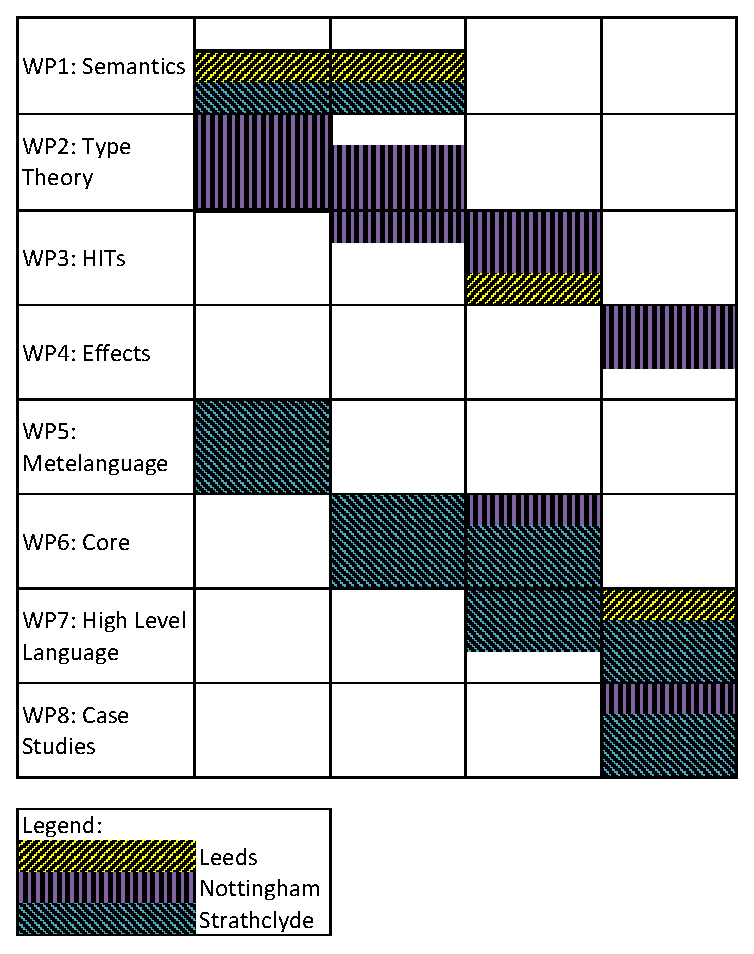
\includegraphics{Gantt.eps}
%\caption{Gantt chart depicting the order and division of work on workpackages}
%\end{figure}
%\newpage

\begin{footnotesize}
\begin{multicols}{2}
\bibliographystyle{plain}
%\bibliographystyle{abbrv}
%\bibliographystyle{plainnat}
\bibliography{proposal,alti,nicola}
\end{multicols}
\end{footnotesize}

% \begin{multicols}{2}
% \bibliographystyle{plain}
% \bibliography{proposal,alti}
% \end{multicols}{2}

\end{document}
